%%%%%%%%%%%%%%%%%%%%%%%%%%%%%%%%%%%%%%%%%%%%%%%%%%%%%%%%%%%%%%%%%%%%%%
\subsection{\label{sec:CondorView-Client-Install}
Installing the CondorView Client Contrib Module} 
%%%%%%%%%%%%%%%%%%%%%%%%%%%%%%%%%%%%%%%%%%%%%%%%%%%%%%%%%%%%%%%%%%%%%%

% We refer to the make_stats program often in this section; make a
% macro for it.
\newcommand{\MakeStats}{\Prog{make\_stats}}

The CondorView Client contrib module is used to automatically generate
World Wide Web (WWW) pages displaying usage statistics of your Condor
Pool.
Included in the module is a shell script which invokes the \Condor{stats}
command to retrieve pool usage statistics from the CondorView server and
generate HTML pages from the results.  
Also included is a Java applet which graphically visualizes Condor 
usage information.  
Users can interact with the applet to customize the visualization and to
zoom in to a specific time frame.
Figure~\ref{fig:view-screenshot} on page~\pageref{fig:view-screenshot}
is a screenshot of a web page created by CondorView.  
To get a further feel for what pages generated by CondorView look like,
you can view the statistics for the University of Wisconsin-Madison pool
by going to URL \Url{http://www.cs.wisc.edu/condor} and clicking on
Condor View.

\begin{figure}[hbt]
\centering
\includegraphics{admin-man/view-screenshot.ps}
\caption{\label{fig:view-screenshot}Screenshot of CondorView Client}
\end{figure}

After unpacking and installing the CondorView Client, a script named
\MakeStats\ can be invoked to create HTML pages displaying Condor usage
for the past hour, day, week, or month.  
By using the Unix \Prog{cron} facility to periodically execute
\MakeStats, Condor pool usage statistics can be kept up to date
automatically.  
This simple model allows the CondorView Client to be easily installed;
no Web server CGI interface is needed.

%%%%%%%%%%%%%%%%%%%%%%%%%%%%%%%%%%%%%%%%%%%%%%%%%%%%%%%%%%%%%%%%%%%%%%
\subsubsection{\label{sec:condorview-client-step-by-step}
Step-by-Step Installation of the CondorView Client}
%%%%%%%%%%%%%%%%%%%%%%%%%%%%%%%%%%%%%%%%%%%%%%%%%%%%%%%%%%%%%%%%%%%%%%

\index{installation!CondorView Client}
\index{CondorView Client!installation}
\begin{enumerate}

\item First, make certain that you have configured a CondorView 
Server~\ref{sec:Contrib-CondorView-Install}
for your pool to log information to disk in order to provide a persistent,
historical database of pool statistics.
The CondorView Client makes queries over the network against this
database.  The \Condor{collector} included with version 6.2.x and 6.1.x
Condor includes this database support.
To activate the persistent database logging, add the following entries into
the configuration file on your central manager: 
\begin{verbatim}
    POOL_HISTORY_DIR = /full/path/to/directory/to/store/historical/data 
    KEEP_POOL_HISTORY = True 
\end{verbatim}
For full details on these and other \condor{collector} configuration file
entries, see section~\ref{sec:Collector-Config-File-Entries} on
page~\pageref{sec:Collector-Config-File-Entries}.

\item Create a directory where CondorView places the
HTML files.  
This directory should be one published by a web server, so HTML
files which exist in this directory can be accessed via a web browser.  
This is referred to as the \File{VIEWDIR} directory.

\item Unpack/untar the CondorView Client contrib module into \File{VIEWDIR}.
This creates several files and subdirectories within \File{VIEWDIR}.

\item Edit the \MakeStats script.  At the top of this file are six parameters
to customize.  The parameters are:

        \begin{description}

	\item[\Macro{ORGNAME}] Set to a brief name identifying
	your organization, for example ``Univ of Wisconsin''.  Do not
	use any slashes in the name or other special regular-expression
	characters. Avoid characters / $\backslash$ \^\ \$.

	\item[\Macro{CONDORADMIN}] Set to the email
	address of the Condor administrator at your site.  
	This email address will appear at the bottom of the web pages.

	\item[\Macro{VIEWDIR}] Set to the full pathname
	(\emph{not} a relative path) to the \File{VIEWDIR} directory selected
	in installation step 2.  
	It is the directory that contains the \MakeStats\ script.

	\item[\Macro{STATSDIR}]  Set to the full
	pathname of the \emph{directory} which contains the \Condor{stats}
	binary.
	The \Condor{stats} program is included in the \Release{bin}
	directory with Condor version 6.1 and above; for Condor version
	6.0x, the \Condor{stats} program can be found in the CondorView
	Server contrib module.  
	The value for \Macro{STATSDIR} is added to the \Macro{PATH}
	parameter by default; see below.  

	\item[\Macro{PATH}] Set to a list of subdirectories,
	separated by colons, where the \MakeStats\ script can find
	\Prog{awk}, \Prog{bc}, \Prog{sed}, \Prog{date}, and \Condor{stats}
	programs.  
	If you have \Prog{perl} installed, set the path to
	include the directory where \Prog{perl} is installed as well.  Using
	the following default works on most systems:
        \begin{verbatim} 
        PATH=/bin:/usr/bin:$STATSDIR:/usr/local/bin
        \end{verbatim}

        \end{description}

\item To create all of the initial HTML files, type
\begin{verbatim}
        ./make_stats setup  
\end{verbatim}
Open the file \File{index.html} to verify things look good.

\index{Condor\_View!use of\Prog{crontab} program}
\index{\Prog{crontab} program}

\item Add the \MakeStats\ program to \Prog{cron}.  
Running \MakeStats\ in step 5 created a \File{cronentries} file.
This \File{cronentries} file is ready to be processed by the Unix
\Prog{crontab} command.
The \Prog{crontab} manual page can familiarize you
with
the \Prog{crontab} command and the \Prog{cron} daemon.
Take a look at the
\File{cronentries} file; by default, it will run 
\Prog{\MakeStats\ hour} every 15 minutes, 
\Prog{\MakeStats\ day} once an hour, 
\Prog{\MakeStats\ week} twice per day, and 
\Prog{\MakeStats\ month} once per day.
These are reasonable defaults.  
You can add these commands to cron on any
system that can access the \MacroU{VIEWDIR} and
\MacroU{STATSDIR} directories,
even on a system that does not have Condor
installed.  The commands do not have to run as user root; in
fact, they should probably not run as root.  These commands can run
as any user that has read/write access to the \File{VIEWDIR}.
To add these
commands to cron, enter : 
\begin{verbatim} 
        crontab cronentries
\end{verbatim}

\item Point your web browser at the \File{VIEWDIR} directory,
and you are finished with the installation.

\end{enumerate}

\index{CondorView!installation|)}
